\chapter{Introducción}

\section{Objetivos del trabajo}

En el presente Trabajo Fin de Máster se analiza la epidemiología de los cánceres de hígado y colon-recto y se detectan genes que permiten identificar tumores.

\begin{itemize}
	\item En el capítulo 1 se presenta la introducción al cáncer y a las ciencias -ómicas.
	\item En el capítulo 2 se describe la epidemiología del cáncer de hígado y colon-recto para comprender el impacto de estos tumores.
	\item En el capítulo 3 se analizan técnicas de \textit{machine learning} con aplicación en transcriptómica.
	\item En el capítulo 4 se detectan genes que permiten diferenciar entre personas sanas y personas con cáncer.
	\item En el capítulo 5 se presenta una aplicación web que permite realizar la detección de biomarcadores.
	\item En el capítulo 6 se muestran las principales conclusiones del trabajo y se muestran líneas abiertas de trabajo.
\end{itemize}

% ---------------------------------

\section{Cáncer}

El cáncer es una enfermedad en la que se produce una división incontrolada de las células \cite{AmericanCancerSociety2015}. Aunque generalmente se habla del cáncer como una única enfermedad, se trata en realidad de un conjunto de enfermedades, existiendo más de 100 tipos distintos de cáncer \cite{NationalCancerInstitute2015}.\\

El cáncer es una enfermedad genética, esto es, causada por cambios en los genes que controlan las funciones celulares \cite{NationalCancerInstitute2015}. Aunque sea genética, en la mayoría de los casos el cáncer no se hereda \cite{Pierce2010}. En general, el proceso de creación del cáncer es complejo y multifactorial: a menudo el causante no es un solo elemento, sino la combinación e interacción de distintos factores ambientales y genéticos \cite{Migliore2012}. \\

Los factores causantes del cáncer se pueden clasificar principalmente en tres categorías:
\begin{enumerate}
	\item Factores no modificables. Son elementos que no se pueden cambiar, como la edad o la herencia genética \cite{WorldHealthOrganization2014, WorldHealthOrganization2020}.
	\item Factores modificables o prevenibles. Algunos ejemplos son el tabaco, el alcohol, la dieta o la exposición a distintos carcinógenos \cite{Cogliano2011}.
	\item Otros factores. Algunas circunstancias no se corresponden a ninguna de las categorías anteriores ya que algunos de sus aspectos no se pueden cambiar. Es el caso de  factores socioeconómicos (como cobertura sanitaria en el lugar de residencia o privación económica) y factores reproductivos u hormonales (como toma de anticonceptivos, lactancia materna o terapia hormonal sustitutiva en mujeres menopáusicas) \cite{WorldHealthOrganization2020}.
\end{enumerate}

A continuación se introducen dos tipos de cáncer con los que se trabajará más adelante: el cáncer de hígado y el cáncer de colon-recto.

% ---------------------------------

\subsection{Cáncer de hígado}

El cáncer de hígado se corresponde con el código C22 de la Clasificación Internacional de Enfermedades, Décima Revisión, integrando las neoplasias malignas de hígado y vías biliares intrahepáticas \cite{ICD10, cie10es}.

\subsubsection{Anatomía y funciones del hígado}

El hígado es el órgano interno más grande y pesado del cuerpo humano, está situado en el cuadrante superior derecho del abdomen, debajo de las costillas, y está compuesto principalmente por dos lóbulos \cite{Abdel-Misih2010}.\\

\newpage
\textbf{Figura 1}. Anatomía del abdomen humano. Ilustración de Ties van Brussel.
\begin{center}
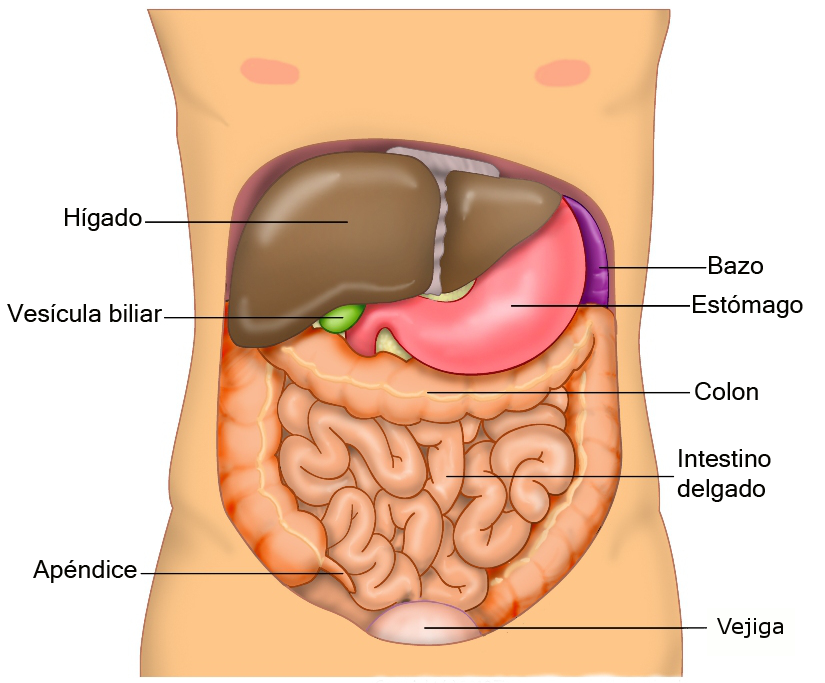
\includegraphics[width=.70\textwidth]{figuras/01_anatomia_higado.png} \\
\end{center}

Las funciones del hígado son múltiples y diversas. Las principales son procesar, particionar y metabolizar macronutrientes, regular el volumen de sangre, apoyar al sistema inmune, eliminar sustancias químicas como el alcohol y otras drogas y producir bilis para absorber grasas \cite{Trefts2017}. Es un órgano imprescindible para la vida.

\subsubsection{Factores de riesgo}

Uno de los factores de riesgo más comunes del cáncer de hígado es la presencia de cirrosis, o sustitución de células sanas de hígado por tejido cicatrizado. La cirrosis puede producirse por varias causas, siendo las más habituales el consumo excesivo de alcohol y la infección con el virus de la hepatitis B o C \cite{AmericanCancerSociety2019}. Otros factores de riesgo son el tabaco, la obesidad, padecer diabetes tipo II y consumir esteroides anabólicos \cite{AmericanCancerSociety2019, Marrero2005}.\\

La prevención del cáncer de hígado se basa en reducir la exposición a factores de riesgo como el tabaco y el alcohol, y en vacunarse contra la hepatitis B \cite{AmericanCancerSociety2019}.

% ---------------------------------

\subsection{Cáncer de colon-recto}

Las neoplasias malignas de colon, recto, unión rectosigmoidea, ano y canal anal (códigos C18-C21 según la Clasificación Internacional de Enfermedades, Décima Revisión \cite{ICD10, cie10es}) a menudo se estudian agrupadas por tener características muy similares.

\subsubsection{Anatomía y funciones del colon-recto}

El colon tiene 3 funciones principales: absorción de agua y electrolitos, producción y absorción de vitaminas y movimiento de heces hacia el recto para su eliminación por el ano \cite{Azzouz2020}.\\

\textbf{Figura 2}. Anatomía del intestino humano. Ilustración de Ties van Brussel.
\begin{center}
	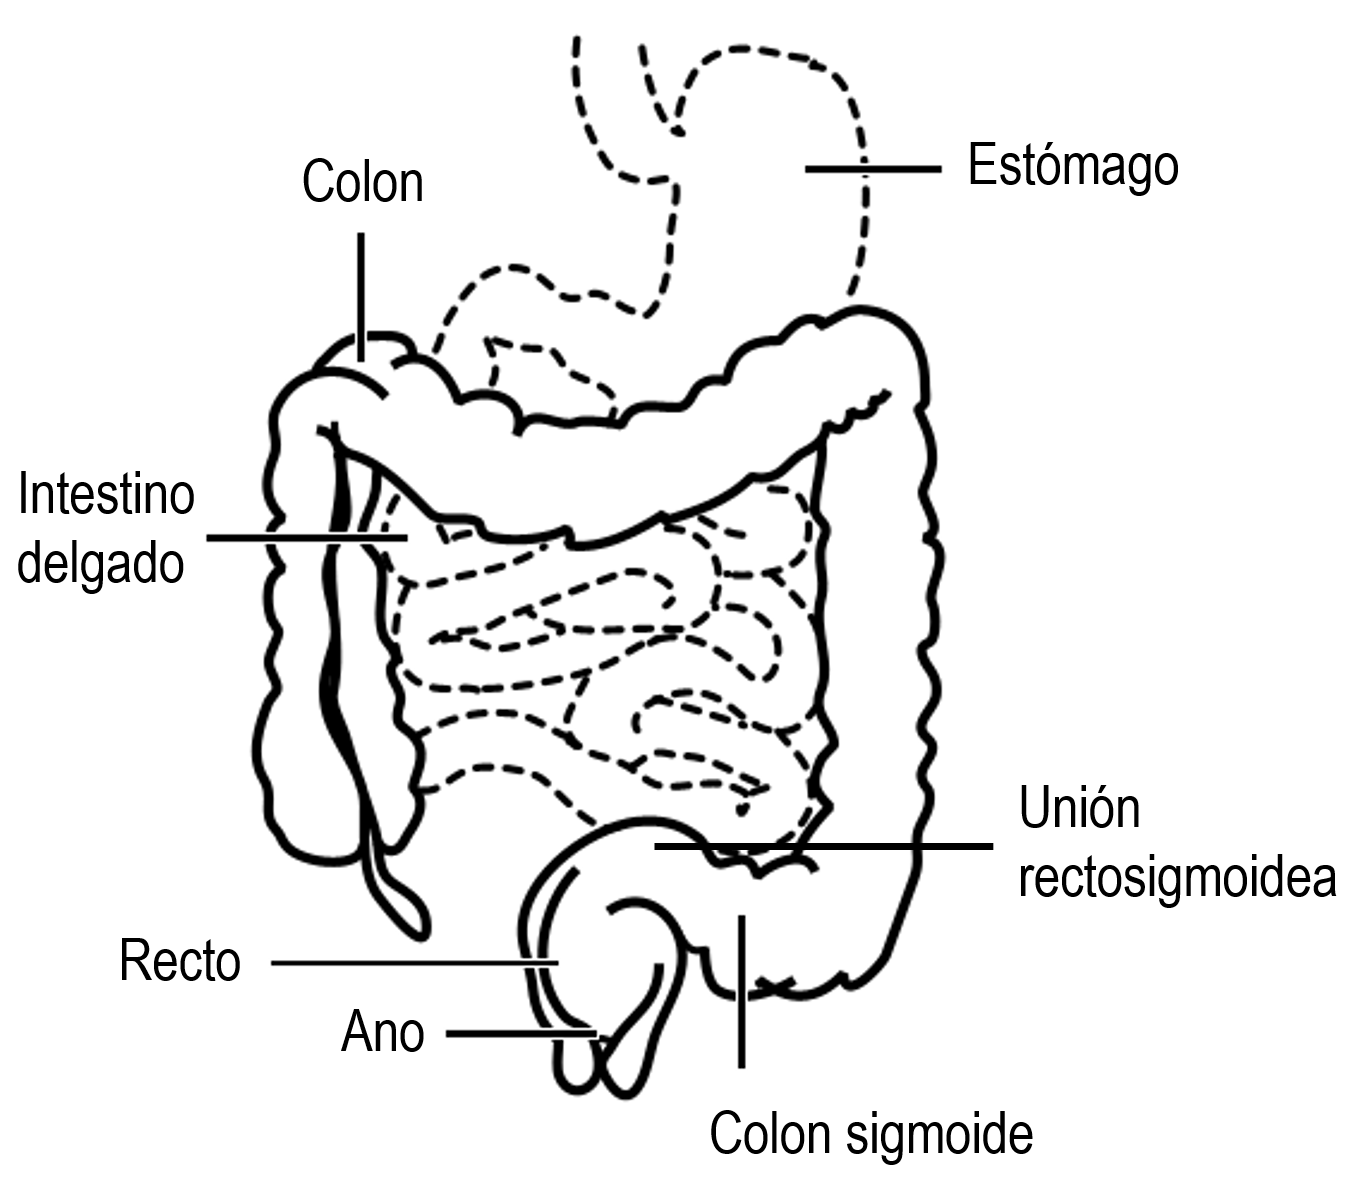
\includegraphics[width=.70\textwidth]{figuras/02_anatomia_cr.png} \\
\end{center}

\subsubsection{Factores de riesgo}

Los factores de riesgo del cáncer de colon-recto  se pueden distinguir en factores modificables y no modificables.\\

Entre los factores de riesgo que son modificables destacan el sobrepeso, la inactividad física, las dietas con alto consumo de carnes rojas o procesadas y el consumo de tabaco y alcohol \cite{AmericanCancerSociety2020}.\\

Algunos factores de riesgo no modificables son una edad superior a 50 años, padecer diabetes tipo 2 y tener antecedentes personales o familiares de cáncer de colon-recto, pólipos o enfermedad intestinal inflamatoria, como colitis ulcerosa y enfermedad de Crohn \cite{AmericanCancerSociety2020}. También existen algunos síndromes hereditarios como el síndrome de Lynch que aumentan las posibilidades de padecer cáncer de colon-recto \cite{Lynch2003}.\\

Para intentar prevenir el cáncer de colon-recto se deben cambiar aquellos factores que son modificables: realizar ejercicio, mantener una dieta saludable y evitar el consumo de tabaco y alcohol. Además, en los últimos años se están implementando programas de cribado de cáncer de colon-recto para detectar pólipos o diagnosticar el cáncer en etapas iniciales mediante análisis como pruebas de sangre oculta en heces o colonoscopias en personas en grupos de riesgo (por ejemplo, mayores de 50 años) \cite{Levin2008}.

% ---------------------------------

\section{Ciencias -ómicas}

Se presenta a continuación una corta introducción a las ciencias -ómicas con el objetivo de comprender los conceptos que se utilizarán más adelante.

\subsection{Introducción a las ciencias ómicas}

Los seres vivos están hechos de células. En el núcleo de cada célula se encuentran los cromosomas, estructuras que almacenan los genes del individuo. Las células humanas tienen 46 cromosomas: 23 heredados de la madre y 23 heredados del padre.\\

La información genética se transporta mediante los ácidos nucleicos: ácido desoxirribonucleico (DNA, por sus siglas en inglés) y ácido ribonucleico (RNA, por sus siglas en inglés). Los ácidos nucleicos son polímeros formados por nucleótidos, que están formados a su vez por un azúcar, un fosfato y una base nitrogenada. En los ácidos nucleicos hay 4 bases nitrogenadas: A, C, G y T para DNA y A, C, G y U para RNA. La información genética se transmite del DNA al RNA, donde se traduce en la secuencia de aminoácidos de una proteína \cite{Pierce2010}.

\subsection{Genómica}

La genómica es la ciencia que estudia la composición, estructura y función de los genomas. Se dedica por tanto a estudiar cromosomas, mutaciones y variaciones tanto de nucleótidos concretos como de regiones del genoma. No debe confundirse con la genética, ciencia que estudia los genes de manera individual \cite{Pierce2010}.\\

El análisis GWAS (Genome-wide association study) es un ejemplo de análisis genómico.

\subsection{Transcriptómica}

La transcriptómica estudia el transcriptoma, esto es, el conjunto de RNA presente en una célula \cite{Schmidt2019}. El transcriptoma indica el nivel de expresión de genes en un determinado momento.\\

Los análisis de RNA-Seq y microRNA son ejemplos de análisis de transcriptómica.\\

Este trabajo se enmarca dentro de la transcriptómica y está basado en datos obtenidos mediante RNA-Seq, técnica en la que se miden distintas lecturas de cada gen para conocer su nivel de expresión, esto es, si los genes están sobreexpresados o infraexpresados, para finalmente comparar esas expresiones con una referencia que suelen ser personas sanas. Como sólo se realizan cuentas de la expresión de los genes, el RNA-Seq de un individuo no permite su identificación, por lo que a menudo estos datos son accesibles de manera abierta.\\

La detección de genes como biomarcadores se ha utilizado ampliamente para intentar predecir el diagnóstico del cáncer, basándose en microarrays \cite{Lee2008, Maglietta2007}, aunque el uso de microarrays está siendo reemplazado por el uso de RNA-Seq  \cite{Stark2019, VanVerk2013}.

\subsection{Otras ciencias -ómicas}

Existen otras ciencias -ómicas, como la proteómica (estudio del proteoma, la imagen dinámica de todas las proteínas expresadas) o la metabolómica (estudio de metabolitos).
